\chapter{Conjuntos de Dados}
\label{sec:aquisicao}

\begin{overview}
  Este capítulo detalha o método de produção dos conjuntos de dados necessários para implementação da classificação automática proposta neste trabalho. A Seção \ref{sec:dados-metodo} descreve a metodologia utilizada para
\end{overview}



% \begin{figure}[!ht]
%   \centering
%   \caption{Fluxograma da aquisição de dados}
%   \label{fig:flow-aquisicao}
%   \simpleflowdiagram{0.6}{
%     Aquisição dos votos do GalaxyZoo (Seção \ref{sec:aquisicao-zoo}),
%     Ajuste do campo de visão angular (Seção \ref{sec:aquisicao-fov}),
%     Aquisição das imagens (Seção \ref{sec:aquisicao-stamps}),
%     Descrição dos conjuntos de dados (Seção \ref{sec:aquisicao-descricao})
%   }
% \end{figure}


\section{Metodologia}
\label{sec:dados-metodo}

\lipsum[1]


\subsection{Aquisição dos Votos do GalaxyZoo}
\label{sec:aquisicao-zoo}

Os votos do GalaxyZoo (Seção \ref{sec:classificacao-cs}) são utilizados como rótulos no treinamento supervisionado do modelo de aprendizagem profunda. Para composição desses rótulos, foram utilizadas sete campanhas do GalaxyZoo: GalaxyZoo 1 \cite{gz1}, GalaxyZoo 2 \cite{gz2,gz2-bias}, GalaxyZoo DECaLS \cite{gz-decals}, GalaxyZoo DESI \cite{gz-desi}, GalaxyZoo Hubble \cite{gz-hubble}, GalaxyZoo Candels \cite{gz-candels} e GalaxyCruisers 1 \cite{gc1}.

Após a aquisição de todos os catálogos de votos, os catálogos foram concatenados e foi feita uma correlação com o próprio catálogo em um raio de 8 arcsec para detecção dos objetos repetidos. Essa etapa de limpeza de dados é essencial, pois um mesmo objeto poderia estar em campanhas distintas do GalaxyZoo e, ao concatenar catálogos de diferentes campanhas, apareceriam objetos duplicados. Isso poderia causar viés na avaliação do modelo, pois, o mesmo objeto poderia aparecer no conjunto de treinamento e de teste/validação simultaneamente.

A Tabela \ref{tab:gz} mostra as estatísticas finais por campanha, após a limpeza dos dados.

\begin{table}[htbp]
  \centering
  \caption{Número de objetos por campanha}
  \label{tab:gz}
  \begin{tabular}{lll}
    \toprule
    \tbh{Campanha}    & \tbh{\# galáxias} & \tbh{\# alternativas} \\
    \midrule
    GalaxyZoo 1       & 93.121            & 6                     \\
    GalaxyZoo 2       & 191.098           & 30                    \\
    GalaxyZoo DESI    & 397.954           & 68                    \\
    GalaxyZoo Hubble  & 92.851            & 40                    \\
    GalaxyZoo Candels & 35.287            & 32                    \\
    \bottomrule
  \end{tabular}
\end{table}







\subsection{Seleção dos Levantamentos Astronômicos}
\label{sec:dados-espectral}


\lipsum[1-2]




\subsection{Ajuste do Campo de Visão Angular}
\label{sec:aquisicao-fov}

O campo de visão angular (em inglês, field of view -- FoV) é a dimensão física da região observada. Essa dimensão é calculada em unidades angulares, pois todas as observações do céu são projetadas na superfície da esfera celeste (Seção \ref{sec:sistema-coordenadas}).

O ajuste do FoV em imagens de galáxias é essencial para o treinamento de modelos baseado em imagens, pois garante que a área da galáxia ocupe uma proporção ideal da imagem. Este ajuste é importante porque afeta diretamente a qualidade das features extraídas, as quais são fundamentais para que o modelo aprenda as características morfológicas das galáxias de forma precisa e consistente. Quando o FoV é ajustado para que a galáxia preencha adequadamente a imagem, o modelo consegue focar nas características principais do objeto, como forma, brilho e estrutura, independentemente de variações no tamanho e na magnitude entre diferentes galáxias.

Se o FoV for proporcionalmente muito pequeno, parte da galáxia pode ser cortada, o que resulta na perda de informações essenciais e introduz inconsistências nas features extraídas, pois o modelo passa a ``ver'' apenas uma parte do objeto. Isso pode levar a erros de classificação ou ao mau desempenho na identificação de padrões morfológicos. Por outro lado, se o FoV for muito grande, a galáxia ocupa uma fração pequena da imagem, e o modelo acaba focando mais no céu ao redor, que é irrelevante para o aprendizado das características morfológicas. Neste segundo caso, a quantidade de pixels dedicados ao fundo dilui a presença da galáxia, dificultando a extração de features relevantes e potencialmente introduzindo ruído nos dados de treinamento.

Foram usadas duas abordagens distintas para estimar automaticamente o FoV para cada galáxia: uma usando o raio efeitivo (Seção \ref{sec:raio-efetivo}) e outra usando a elipticidade complexa (Seção \ref{sec:elipticidade}). Em ambos os casos, os valores são corrigidos por uma função $\eta$ que depende da magnitude da galáxia (Seção \ref{sec:magnitude}) na banda r. Essa função foi ajustada empiricamente com base na inspeção visual. As medidas de raio efetivo, elipticidade complexa e magnitude foram obtidas do catálogo fotométrico do Legacy Survey (Seção \ref{sec:legacy}) acessadas a partir do AstroDataLab (\url{https://datalab.noirlab.edu}) pelo protocolo TAP (Seção \ref{sec:protocolos}).

A estimativa do FoV a partir do raio efetivo foi inspirada pelo método desenvolvido por \citeonline{gz-decals}. Neste caso, consideramos que a região vista na figura deve conter o dobro do raio efetivo (diâmetro efetivo) corrigido por uma função $\eta$ (explicada mais adiante) que depende da magnitude ($r_\mathrm{mag}$), como mostra a eq. \eqref{eq:fov-circ}.

\begin{equation}\label{eq:fov-circ}
  \mathrm{fov}_c = 2 \cdot r_e \cdot \eta(r_\mathrm{mag})
\end{equation}

A segunda abordagem consiste na estimativa do FoV a partir da elipticidade expressa pelo número complexo da eq. \eqref{eq:ellip-complex}. O catálogo fotométrico do Legacy Survey (Seção \ref{sec:legacy}) fornece os valores das componentes real ($\epsilon_1$) e imaginária ($\epsilon_2$).

\begin{equation}\label{eq:ellip-complex}
  \epsilon = \frac{a-b}{a+b} e^{2i\phi} = \epsilon_1 + i\epsilon_2
\end{equation}


A partir dos valores das componentes $\epsilon_1$ e $\epsilon_2$, é calculado o módulo do elipticidade ($|\epsilon|$), conforme a eq. \eqref{eq:mod}.

\begin{equation}\label{eq:mod}
  |\epsilon| = \sqrt{\epsilon_1^2 + \epsilon_2^2}
\end{equation}

Com o valor do módulo, os valores dos semi-eixos maior e menor ($a$ e $b$, respectivamente) e do ângulo ($\phi$) da elípse são calculados pelas eqs. \eqref{eq:b/a} e \eqref{eq:phi}.

\begin{equation}\label{eq:b/a}
  \frac{b}{a} = \frac{1 - |\epsilon|}{1 + |\epsilon|}
\end{equation}

\begin{equation}\label{eq:phi}
  \phi = \frac{1}{2}\arctan\frac{\epsilon_2}{\epsilon_1}
\end{equation}

O próximo passo é calcular a caixa delimitadora (\emph{bounding box}) da elipse. Para fazer isso, usamos as equações paramétricas da elípse, conforme as eqs. \eqref{eq:x(t)} e \eqref{eq:y(t)}.

\begin{equation}\label{eq:x(t)}
  x(t) = x_0 + \frac{a}{2} \cos t \cos\phi - \frac{b}{2} \sin t \sin\phi
\end{equation}

\begin{equation}\label{eq:y(t)}
  y(t) = y_0 + \frac{b}{2} \sin t \cos\phi + \frac{a}{2} \cos t \sin\phi
\end{equation}

Então, expressamos o parâmetro $t$ em termos os semi-eixos e do ângulo, como as eqs. \eqref{eq:tx} e \eqref{eq:ty}.

\begin{equation}\label{eq:tx}
  t_x = \arctan\left(-\frac{b\tan\phi}{a}\right)
\end{equation}

\begin{equation}\label{eq:ty}
  t_y = \arctan\left(\frac{b}{a\tan\phi}\right)
\end{equation}

Então, considerando o ponto $(x_0, y_0)$ como as coordenadas do centro da imagem, em pixels, obtemos as quatro coordenadas da caixa delimitadora da elípse $x_1$, $x_2$, $y_1$ e $y_2$, em pixels, como mostra a eq. \eqref{eq:bb}.

\begin{equation}\label{eq:bb}
  x_1 = x(t_x) \qquad x_2 = x(t_x + \pi) \qquad y_1 = y(t_y) \qquad y_2 = y(t_y + \pi)
\end{equation}

A caixa delimitadora da elípse é um retângulo. No entanto, queremos que as imagens das galáxias sejam quadradas, então calculamos o lado do quadrado $\ell$, conforme a eq. \eqref{eq:l}.

\begin{equation}\label{eq:l}
  \ell = \max(|x_2 - x_1|, |y_2 - y_1|)
\end{equation}

Finalmente, calculamos o FoV pela eq. \eqref{eq:fov-ellip}

\begin{equation}\label{eq:fov-ellip}
  \mathrm{fov}_e = \ell \cdot \eta(r_{\mathrm{mag}})
\end{equation}

É notável que um valor $\eta$, usado como fator de correção, foi usado em ambas as abordagens. Foi necessário porque é necessário escalonar as medidadas de raio efetivo e elipticidade para que seja possível usá-las como estimativa do FoV. No entanto, o valor depende da magnitude: para objetos mais brilhantes, deve-se multiplicar por um valor maior que para objetos menos brilhantes.

Desse modo, foi considerado um intervalo de $r_{\mathrm{mag}}$ entre 8 e 20 e foram amostradas 500 galáxias para cada intervalo de 1 mag (12 amostras). Sendo que, para os intervalos mais brilhantes, foram obtidas menos de 500 galáxias. Para cada intervalo de magnitude, foram atribuídos valores de ajuste para ambas as abordagens. Assim, a função $\eta$ foi empiricamente determinada por inspeção visual de amostras aleatórias de galaxias em intervalos de magnitude, como mostra a Fig. \ref{fig:eta}. Por critério de documentação, a inspeção visual realizada está disponível na página \url{https://nmcardoso.github.io/ls-stamps}, contendo todos os ajustes para todas as galáxias inspecionadas.

\begin{figure}[!ht]
  \centering
  \caption{Fator de correção ($\eta$) ajustado por inspeção visual}
  \label{fig:eta}
  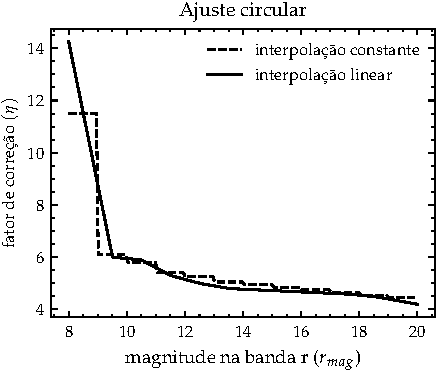
\includegraphics[width=0.51\linewidth]{notebooks/plots/correction_factor_circ.pdf}\hfill
  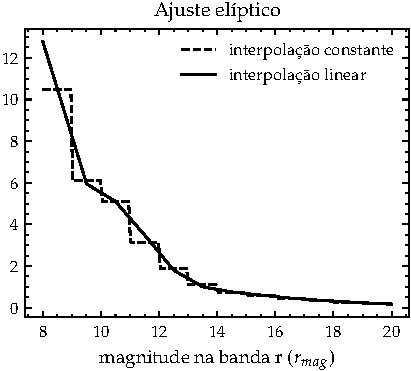
\includegraphics[width=0.48\linewidth]{notebooks/plots/correction_factor_ellip.pdf}
\end{figure}


O processo de ajuste do FoV é exemplificado nas figs. \ref{fig:fov-stamps-1} e \ref{fig:fov-stamps-2}. Nelas, são mostrados os ajustes de 12 galáxias, uma para cada intervalo de magnitude, tanto para o ajuste circular (primeiro método) quanto para o ajsute elíptico (segundo método). No ajuste circular, a circunferência indica o raio efetivo da galáxia escalonado pela função $\eta$. Analogamente, no ajuste elíptico, a elípse é obtida pelos parâmetros calculados nas eqs. \eqref{eq:b/a} e \eqref{eq:phi} escalonados pela função $\eta$, e o retângulo tracejado indica a caixa delimitadora da elípse, cujos limites são obtidos da eq. \eqref{eq:bb}. Em ambas as colunas, o quadrado branco indica o FoV calculado em cada caso, de acordo com as eqs. \eqref{eq:fov-circ} e \eqref{eq:fov-ellip}. As colunas ``corte circular'' e ``corte elíptico'' mostram as figuras finais após o ajuste pelo método do raio efetivo e da elipsidade complexa, respectivamente. A região vista nessas colunas é equivalente à região delimitada pelos quadrados brancos nas colunas de ajuste. Para comparação entre os métodos, ambas as colunas de ajuste possuem o mesmo FoV, definido manualmente para cada intervalo de magnitude.

Analisando os ajustes com o método do raio efetivo, notamos que há uma tendencia dessa abordagem subestimar o FoV de galáxias grandes, distorcidas ou de sistemas de galáxias, como mostra os Objetos 3 ao 6 da Fig. \ref{fig:fov-stamps-1} e o Objeto 7 da Fig. \ref{fig:fov-stamps-2}, além de sobre-estimar o FoV de galáxias menos brilhantes, como os Objetos 10 e 11 da Fig. \ref{fig:fov-stamps-2}. Por outro lado, o método da elípse pareceu mais consistente para determinação dos FoVs e por isso foi o método escolhido.

\begin{figure}[!ht]
  \centering
  \caption{Ajuste do campo de visão angular para $r_{mag}$ entre 8 e 13}
  \label{fig:fov-stamps-1}
  \includegraphics[width=0.99\linewidth]{notebooks/plots/stamps_crop_1.pdf}
\end{figure}

\begin{figure}[!ht]
  \centering
  \caption{Ajuste do campo de visão angular para $r_{mag}$ entre 14 e 19}
  \label{fig:fov-stamps-2}
  \includegraphics[width=0.99\linewidth]{notebooks/plots/stamps_crop_2.pdf}
\end{figure}








\subsection{Aquisição das Imagens}
\label{sec:aquisicao-stamps}

A aquisição dos pequenos recortes de imagens astronômicas centrados em objetos específicos (stamps) do Legacy Survey por meio do serviço Hips2Fits\footnote{\url{https://alasky.cds.unistra.fr/hips-image-services/hips2fits}} \cite{aladin}, do Strasbourg Astronomical Data Center\footnote{\url{https://cds.unistra.fr}} (CDS), envolve um processo meticuloso de coleta de imagens ajustadas para um grande número de galáxias. Considerando que os campos de visão (FOVs) de cada objeto foram previamente calculados para garantir que a área da galáxia ocupe uma proporção ideal na imagem, a aquisição pode então ser automatizada, eficiente e escalável. Para realizar essa aquisição em larga escala, que pode envolver milhões de galáxias, é fundamental utilizar uma arquitetura de paralelização eficiente, como o modelo de produtor-consumidor, combinada com mecanismos de controle de taxa de requisição, mostrado na Fig. \ref{fig:stamps-sequence}.

\begin{figure}[!ht]
  \centering
  \caption{Diagrama de sequência da arquisição das imagens}
  \label{fig:stamps-sequence}
  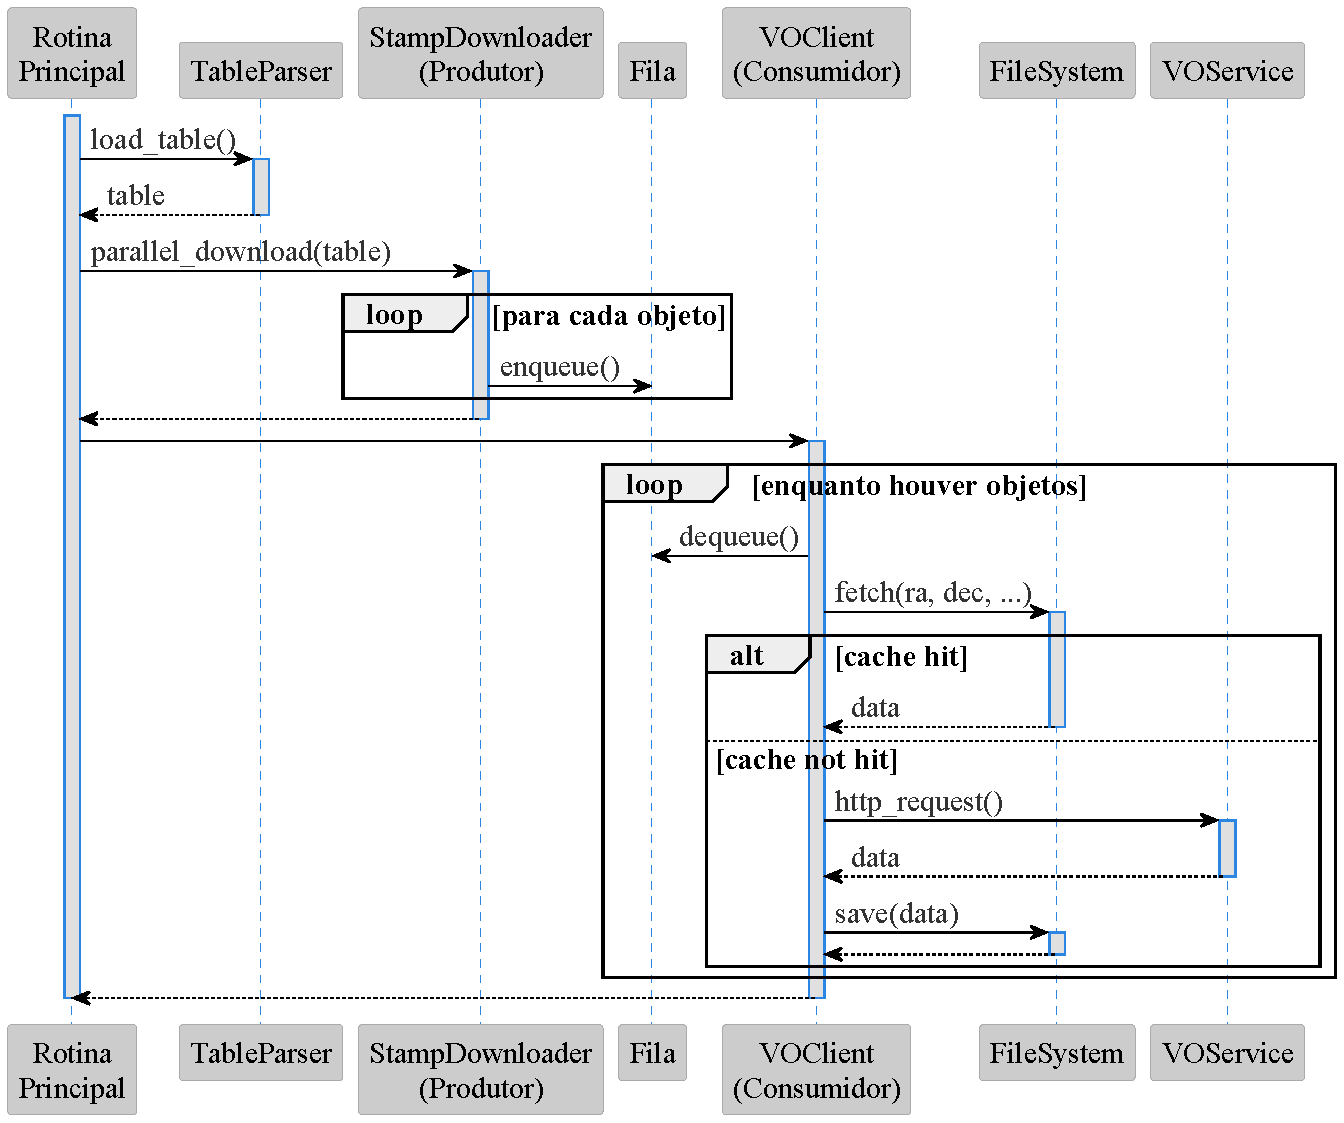
\includegraphics[width=\linewidth]{diagrams/plots/sequence.pdf}
\end{figure}


Inicialmente, o sistema é projetado em duas camadas principais: a camada de produtores, responsáveis por gerar as requisições de imagens para cada galáxia com seu respectivo FOV, e a camada de consumidores, encarregada de processar essas requisições e armazenar os stamps retornados. No caso de uma grande quantidade de objetos, é necessário implementar várias threads que operem de forma concorrente para maximizar o desempenho e a eficiência do sistema. Os produtores criam as requisições HTTP para o Hips2Fits, especificando os parâmetros de coordenadas do objeto (como RA e Dec) e o FOV calculado. Esses parâmetros garantem que a imagem adquirida seja adequada à análise morfológica planejada.

A arquitetura paralela é gerenciada com o uso de um semáforo, um mecanismo de controle de concorrência que limita o número de requisições simultâneas feitas ao servidor Hips2Fits. Esse semáforo é configurado de acordo com a taxa de requisição máxima permitida pelo servidor, evitando sobrecarga e bloqueios temporários ou permanentes impostos pelo controle de acesso ao servidor. O semáforo atua para que um número limitado de threads possa realizar requisições ao mesmo tempo; assim, ao alcançar o limite, novas requisições aguardam até que uma thread finalize seu processo e libere o semáforo para outra requisição.

Esse modelo de produtor-consumidor com controle de taxa de requisição não apenas respeita os limites de acesso do Hips2Fits, mas também assegura uma coleta eficiente e escalável. Como cada thread pode solicitar e processar imagens independentemente, o tempo total de execução é significativamente reduzido, permitindo a aquisição dos stamps para milhões de galáxias em um tempo viável. Essa abordagem de paralelização e controle de acesso torna o sistema robusto para grandes volumes de dados, possibilitando o processamento em lotes de imagens astronômicas de forma a atender à demanda de análise em larga escala na pesquisa astronômica.












\section{Conjuntdo de Referência}
\label{sec:dados-referencia}



\subsection{Pipeline de Dados}
\label{sec:dados-pipeline}

\lipsum[1-2]

\begin{figure}[h!]
  \centering
  \caption{Pipeline de produção do catálogo de referência}
  \label{fig:pipeline-ref}
  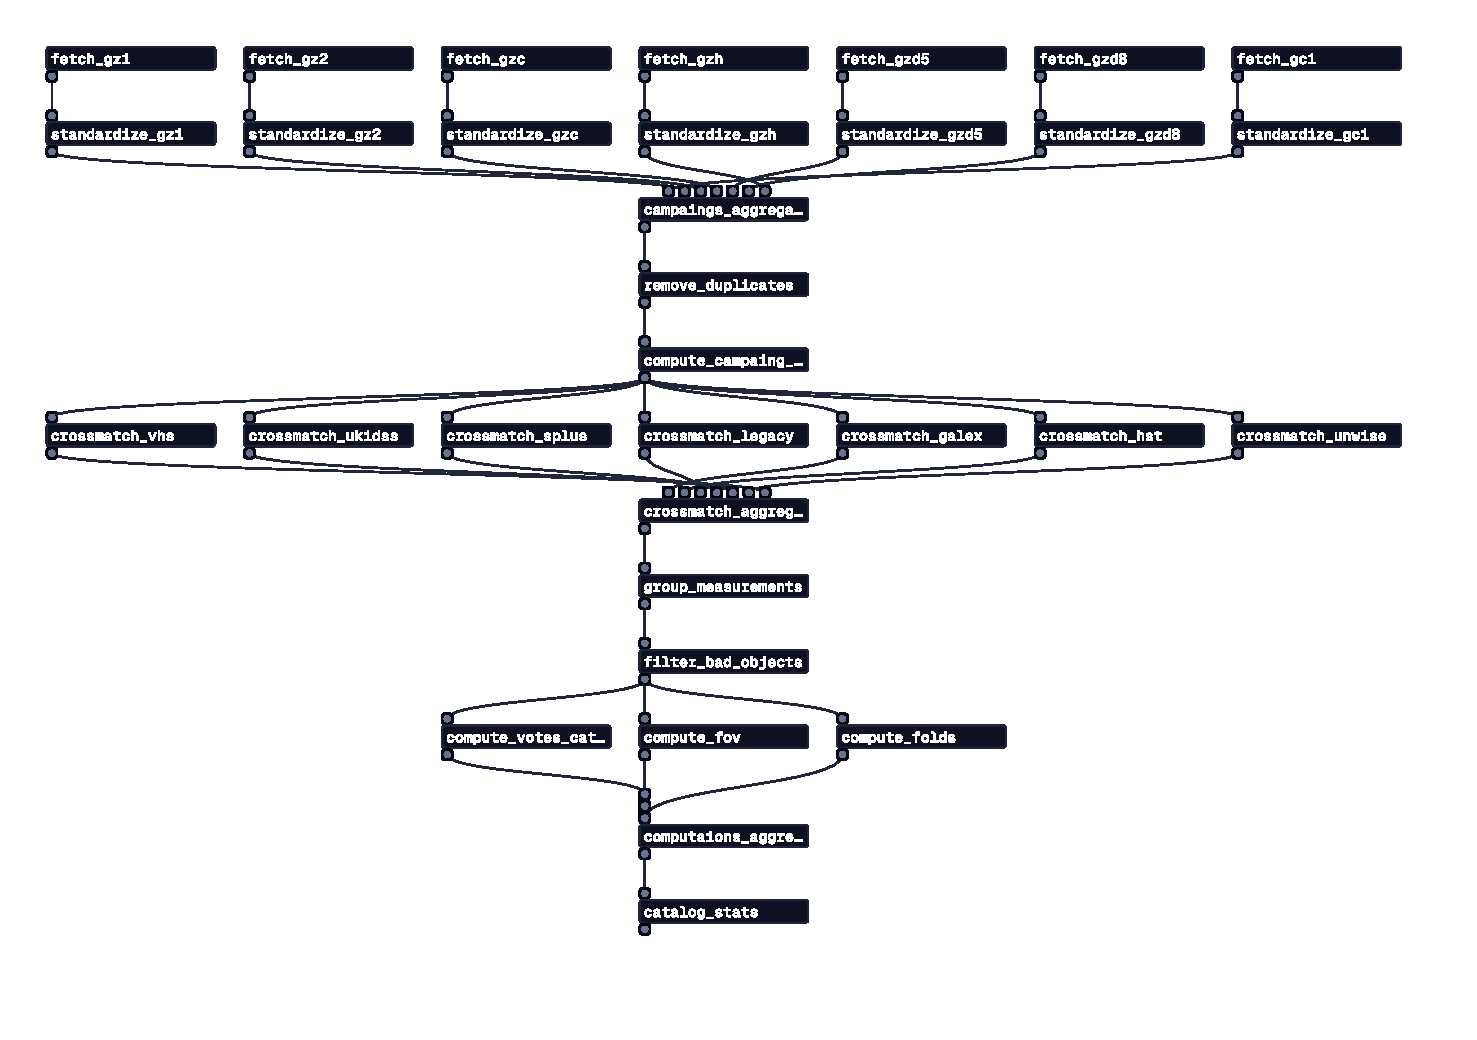
\includegraphics[width=\linewidth,trim={8mm 20mm 15mm 8mm},clip]{figures/pipe.pdf}
\end{figure}




\subsection{Descrição}
\label{sec:aquisicao-descricao}

Nesta Seção, é feita uma análise, de forma agregada, sobre as propriedades físicas das galáxias dos conjuntos de dados para garantir a coerência no treinamento do modelo.

\subsubsection{Conjuntos de Treinamento, Validação e Teste}
\label{sec:aquisicao-treinamento}

Garantir que os conjuntos de treinamento, validação e teste possuam distribuições similares de magnitude (Fig. \ref{fig:conjuntos_magr}) e campo de visão angular (Fig. \ref{fig:conjuntos_fov}) é crucial para o treinamento do modelo. Distribuições consistentes asseguram que o modelo seja exposto a dados representativos durante o treinamento, prevenindo vieses que poderiam comprometer sua capacidade de generalizar para novos dados. Magnitudes diferentes podem indicar variações no brilho dos objetos, influenciando os padrões visuais extraídos pelos modelos, enquanto campos de visão angulares distintos podem alterar o contexto espacial e os detalhes observados. Desequilíbrios entre esses conjuntos podem levar a discrepâncias na avaliação, onde métricas de desempenho no conjunto de teste não refletem a eficácia real do modelo em aplicações práticas.

\begin{figure}[!ht]
  \centering
  \caption{Distribuição da magnitude na banda r}
  \label{fig:conjuntos_magr}
  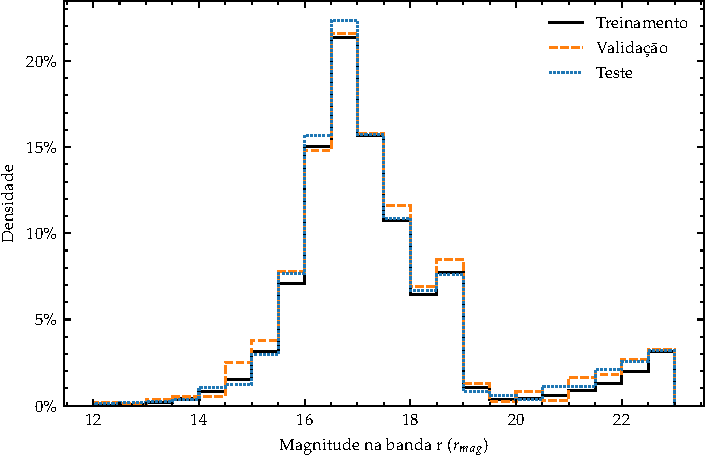
\includegraphics[width=\linewidth]{notebooks/plots/conjuntos_magr.pdf}
\end{figure}


\begin{figure}[!ht]
  \centering
  \caption{Distribuição do campo de visão angular}
  \label{fig:conjuntos_fov}
  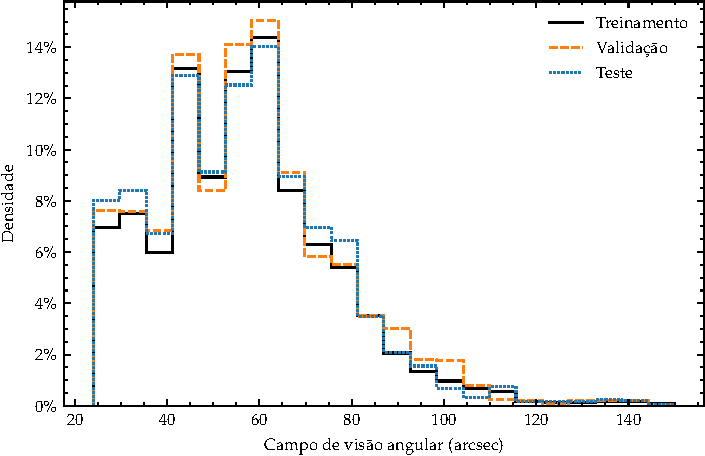
\includegraphics[width=\linewidth]{notebooks/plots/conjuntos_fov.pdf}
\end{figure}







\subsubsection{Conjunto de Inferência}
\label{sec:aquisicao-inferencia}

\subsection{Pipeline de Dados}
\label{sec:dados-inferencia-pipeline}

\lipsum[1-2]

\begin{figure}[h!]
  \centering
  \caption{Pipeline de produção do catálogo de referência}
  \label{fig:pipeline-ref}
  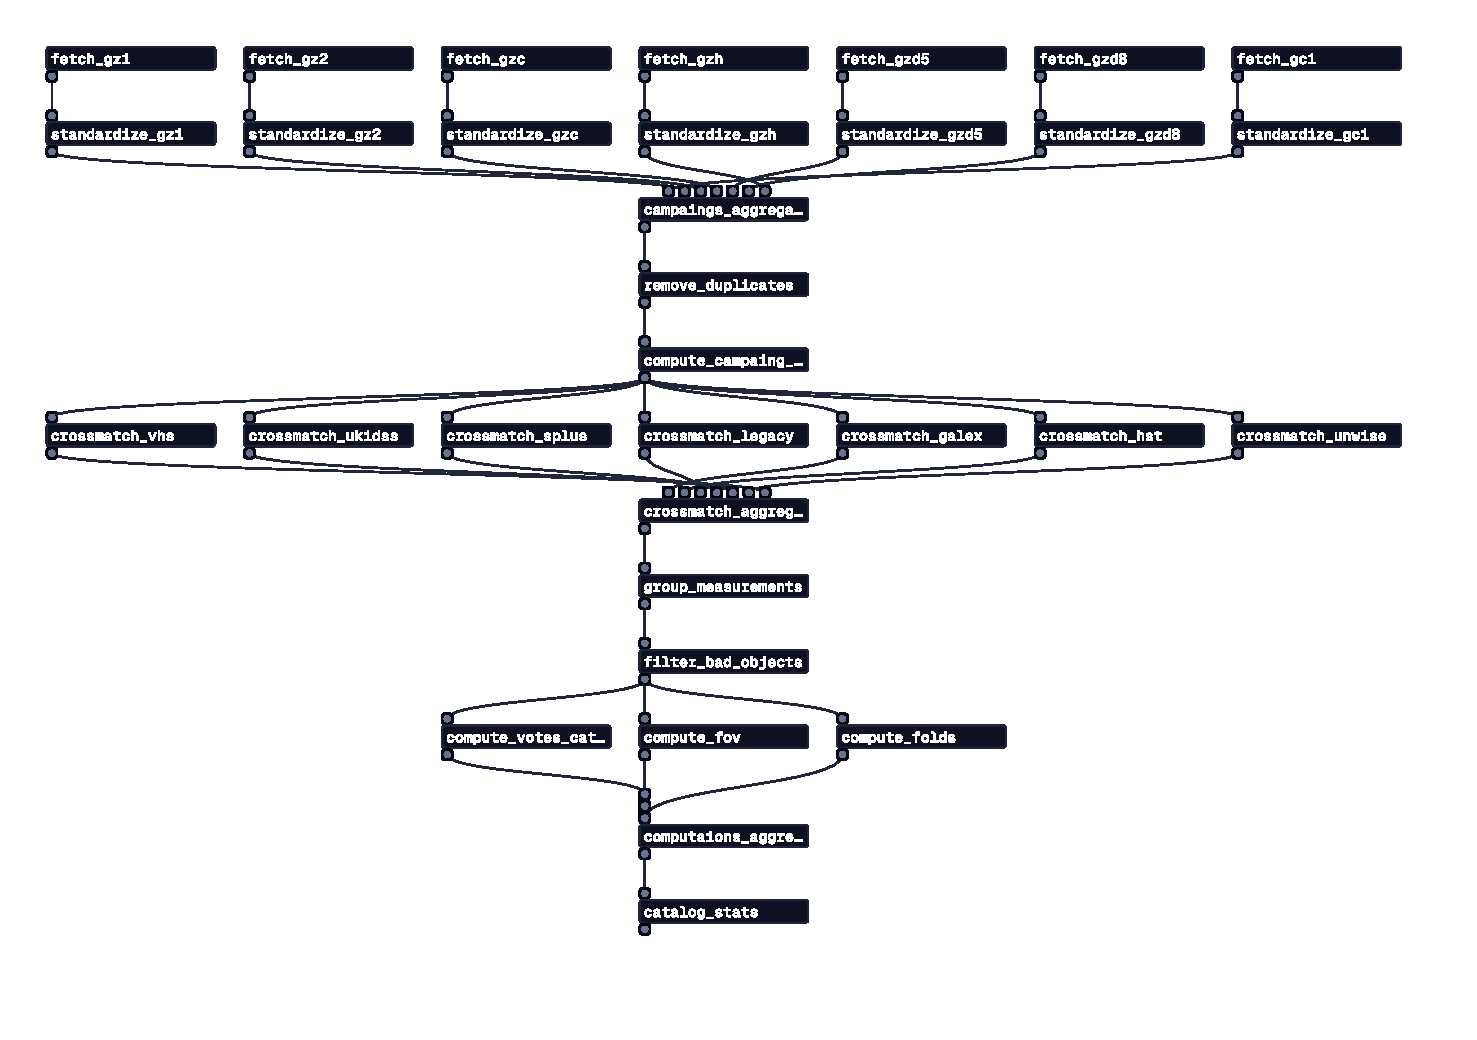
\includegraphics[width=\linewidth,trim={8mm 20mm 15mm 8mm},clip]{figures/pipe.pdf}
\end{figure}






\subsection{Descrição}
\label{sec:dados-inferencia-descricao}
O conjunto de inferência é formado por aproximadamente 8 milhões de objetos. A Fig. \ref{fig:conjuntos_inferencia} mostra a distribuição espacial das galáxias, em que as cores codificam a densidade de galáxias em uma determinada região, conforme mostrado na escala.

\begin{figure}[!ht]
  \centering
  \caption{Área de cobertura espacial do conjunto de inferência}
  \label{fig:conjuntos_inferencia}
  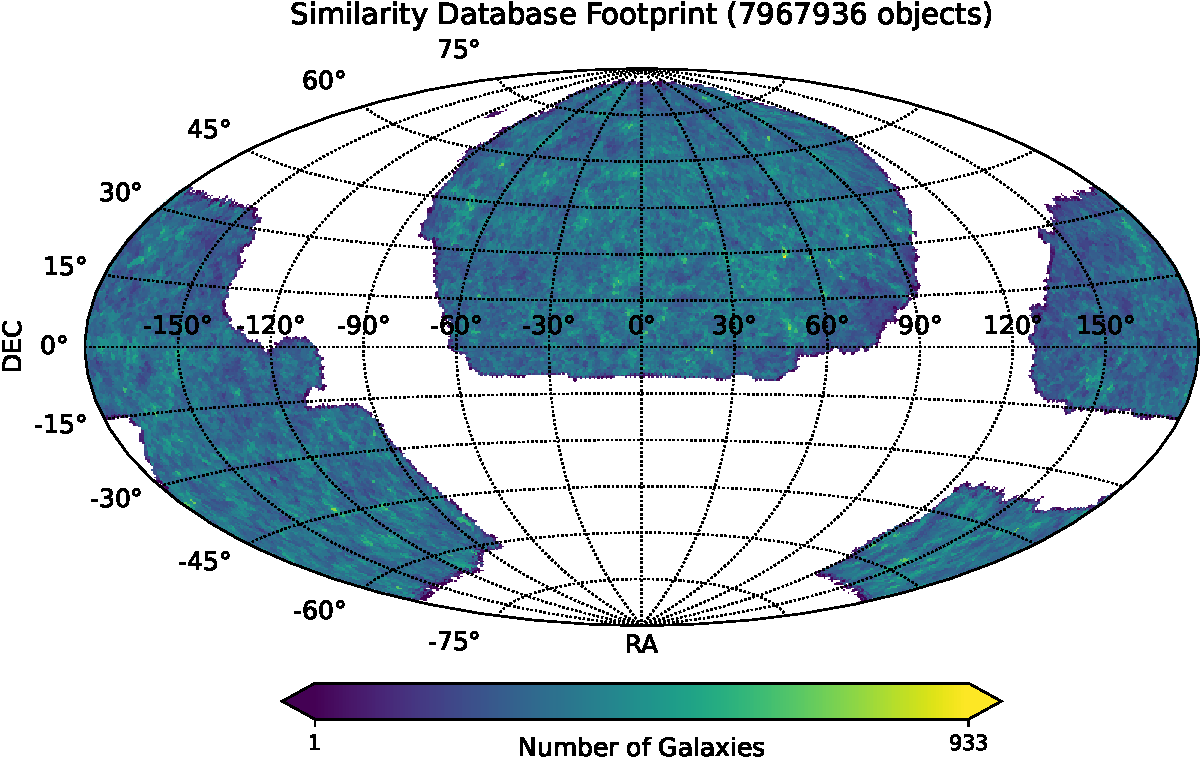
\includegraphics[width=\linewidth]{figures/similarity_footprint.pdf}
\end{figure}


Os conjuntos de treinamento e inferência utilizados neste trabalho, composto por 400 mil e 8 milhões de imagens obtidas do DESI Legacy Survey, respectivamente, possuem uma longa durabilidade científica devido às características intrínsecas do levantamento e ao tipo de observação realizada. Como um levantamento de campo profundo e não transiente, o Legacy Survey foca na captura de objetos celestes distantes e estáticos, como galáxias e aglomerados de galáxias, que não apresentam variações significativas em escalas temporais humanas. Esses objetos, frequentemente dominados por matéria escura, são fundamentais para o estudo da evolução cósmica e da distribuição de massa no universo em larga escala. A natureza estável dessas observações permite que os dados permaneçam relevantes por décadas, fornecendo uma base sólida para análises contínuas e complementares, à medida que novos modelos de aprendizado profundo e técnicas de análise de dados são desenvolvidos. Essa durabilidade é particularmente valiosa em um contexto científico onde as demandas computacionais e as abordagens metodológicas evoluem rapidamente, garantindo que o conjunto de inferência continue a contribuir para avanços na pesquisa astronômica e cosmológica.

Esta análise encerra a seção de descrição dos dados. A seguir, serão detalhados os métodos de aprendizado profundo utilizados para o treinamento do modelo.





\chaptersep
